```latex
\begin{document} 

\maketitle

\begin{abstract}
  Este artigo documenta os aspectos práticos da implementação de soluções
  para o Problema do Caixeiro Viajante, um problema bem conhecido e difícil que requer
  tempo exponencial para encontrar a solução ótima. Foram implementados três algoritmos:
  uma solução exata através da técnica de branch-and-bound, e duas outras aproximações,
  os algoritmos twice-around-the-tree e Christofides.
\end{abstract}
     
\begin{resumo} 
  Este artigo documenta os aspectos práticos da implementação de soluções
  para o Problema do Caixeiro Viajante, um problema bem conhecido e difícil que requer
  tempo exponencial para encontrar a solução ótima. Foram implementados três algoritmos:
  uma solução exata através da técnica de branch-and-bound, e duas outras aproximações,
  os algoritmos twice-around-the-tree e Christofides.
\end{resumo}


\section{Introdução ao Problema do Caixeiro Viajante} \label{sec:intro}

O Problema do Caixeiro Viajante (TSP) é adequadamente descrito por \cite{brilliant_explanation} 

\begin{quote}
  "Um vendedor precisa visitar um conjunto de cidades para vender seus produtos. Eles sabem quantas 
  cidades precisam visitar e as distâncias entre cada cidade. Em que ordem 
  o vendedor deve visitar cada cidade exatamente uma vez para minimizar seu 
  tempo de viagem e para que termine sua jornada em sua cidade de origem?"
\end{quote}

O TSP é um \textbf{problema intratável} bem conhecido, o que, no contexto de 
algoritmos, significa que o tempo e/ou espaço necessário para resolver o problema cresce 
exponencialmente com o tamanho da entrada, tornando impraticável resolvê-lo mesmo para 
entradas relativamente pequenas.

Este projeto documenta o desenvolvimento de três soluções para o problema em questão, 
focando na avaliação dos desafios do mundo real associados a elas, como planejamento e 
otimização, tomada de decisões informadas sobre estruturas de dados e bibliotecas, e 
análise do uso de recursos computacionais.

\section{Algoritmos} \label{sec:algoritmos}

O problema TSP pode ser convenientemente modelado por um grafo ponderado, sendo os nós do grafo 
as cidades e os pesos das arestas especificando as distâncias.

Para resolvê-lo, três algoritmos foram implementados neste projeto: uma solução ótima usando 
a técnica de branch-and-bound, e duas aproximações, os algoritmos twice-around-the-tree e o 
algoritmo de Christofides.

\subsection{Solução Ótima} \label{sec:optimal_explanation}

O branch and bound é um método geral que tenta dividir um problema em subproblemas menores,
e então toma decisões informadas para descartar alguns desses subproblemas para alcançar a solução ótima.

Ao considerá-lo no contexto do TSP, beneficia-se de \textbf{visualizar o problema como uma árvore}, onde cada nó 
representa uma cidade e cada aresta um caminho entre duas cidades. Então, o primeiro nó pode ser qualquer cidade 
(já que se pode começar de qualquer cidade do caminho ótimo sem alterar a distância do caminho), e 
o caminho do nó de origem até uma folha na árvore deve representar o comprimento total 
daquele caminho.

No entanto, simplesmente armazenar a árvore inteira evidentemente resultaria em uma quantidade enorme 
de dados, já que todas as combinações possíveis acabariam sendo armazenadas na memória. É por isso que o 
método de branch and bound deve tomar a decisão de qual cidade visitar em seguida com base em todas as decisões 
anteriores, o que pode ser chamado de \textbf{limite inferior}.

O parâmetro de limite inferior para selecionar a próxima cidade é calculado somando a 
distância do caminho atual com a distância mínima para qualquer cidade não visitada. Mantendo essa métrica 
para cada caminho parcial, o algoritmo de branch and bound descarta subproblemas que não podem 
levar à solução ótima, concentrando-se efetivamente nos caminhos mais promissores.

Além disso, pode-se fazer uma escolha sobre qual método utilizar para percorrer o "espaço" de possibilidades: \textbf{best-first-search} ou \textbf{depth-first-search}. A variedade \textit{best} significa que o caminho de cada cidade vizinha será calculado antes de fazer uma escolha, o que permitirá ao algoritmo tomar decisões mais informadas para descartar os ramos, mas exigirá mais memória. Em segundo lugar, a variedade \textit{depth} de travessia é a busca padrão que se aprofunda na árvore, o que exigirá menos espaço, mas pode levar mais tempo percorrendo os ramos. Como esta é uma abordagem dispendiosa, foi escolhido o DFS.

A técnica de branch and bound tem uma complexidade de tempo no \textbf{pior caso} de $O(n!)$, 
onde $n$ é o número de cidades, pois pode ser necessário explorar todas as permutações possíveis. 
No entanto, a limitação eficaz pode reduzir significativamente o número de permutações examinadas, 
tornando-o mais eficiente do que uma abordagem ingênua de força bruta. O desempenho real depende da 
instância específica do problema e da técnica de limitação utilizada.

\subsection{Solução Aproximada: Christofides} \label{sec:chris_explanation}

O algoritmo de Christofides foi desenvolvido aproveitando uma percepção-chave: muitas das arestas na 
solução ótima são frequentemente encontradas na Árvore de Abrangência Mínima (MST) do mesmo grafo 
\footnote{\cite{reducible_explanation}}. Portanto, como existem algoritmos relativamente eficientes 
para gerar a MST, faz sentido tentar aproveitar esse fato.

Para formar uma solução ótima, todos os nós da MST devem ter um número par de arestas, para que 
o vendedor possa entrar e sair da cidade por exatamente duas arestas (também conhecido como um 
\textit{Eulerian Tour}). No entanto, a maioria das MSTs possui nós com um número ímpar de arestas, 
o que exigirá a adição de mais arestas.

A segunda parte da solução envolve encontrar boas candidatas a arestas para adicionar às arestas 
ímpares. De várias opções disponíveis, a abordagem usada nesta implementação foi a correspondência 
de comprimento mínimo dos nós de grau ímpar, que tenta encontrar uma correspondência máxima em um grafo 
bipartido com peso total mínimo. Em outras palavras, tenta encontrar os melhores nós (distância mais curta) 
que conectam cada par de nós de grau ímpar da

 MST.

Combinando a MST com a correspondência de comprimento mínimo, obtemos uma aproximação muito boa 
da solução ótima do TSP, que pode ser facilmente construída percorrendo esse grafo, tomando atalhos 
para evitar visitar várias cidades.

De acordo com \cite{Johnson2003}, o algoritmo de Christofides oferece uma garantia de \textbf{pior caso} melhor 
do que qualquer outra heurística de construção de circuitos conhecida: uma razão de pior caso de 1,5; 
[e] também tende a encontrar circuitos melhores na prática. No entanto, calcular a correspondência 
de comprimento mínimo nos vértices de grau ímpar continua sendo o gargalo do algoritmo.

\subsection{Solução Aproximada: Twice Around the Tree} \label{sec:twice_explanation}

O Twice-around-the-tree também usa a MST para gerar uma solução. A ideia é gerar um caminho 
através desta MST, percorrendo-a duas vezes, uma vez em cada direção (o que significa que as cidades 
podem ser visitadas mais de uma vez). Isso pode ser feito por uma travessia em profundidade (DFS).

Para melhorar a qualidade da solução, o algoritmo TAT tenta encurtar o 
caminho adicionando arestas extras a ele. Essas arestas são escolhidas de tal forma que reduzam 
o comprimento total do caminho. O algoritmo continua a adicionar arestas até que o comprimento 
do caminho não mude significativamente.

Este algoritmo tem uma garantia de \textbf{pior caso} de 2 (também chamada de \textit{2-aproximada}), o que significa 
que o custo total do caminho encontrado é no máximo duas vezes o custo da MST.

É possível implementar uma otimização e alcançar um algoritmo semelhante ao \textit{Approx-TSP-Tour} 
descrito por \cite{cormen}, e essa abordagem possui complexidade polinomial: sua complexidade é $number\_of\_cities^2^2$.


\section{Escolhas de Implementação e Instruções de Execução} \label{sec:implementation}

A linguagem de programação utilizada foi o Python 3.12, e o programa foi executado 
em um Ambiente Virtual Python na distribuição Linux Ubuntu 23.10, em um computador com um 
processador Intel Core i5-4690K e 8 GB de RAM a 2133 MHz.

Os \textbf{conjuntos de dados} foram selecionados pelo professor a partir do TSPLIB \cite{dataset_lib}. Eles são 
compostos por arquivos \texttt{.tsp} com a chave do nó e sua localização $x$ e $y$ no plano cartesiano. 
Os grafos devem ser construídos considerando que todas as cidades estão conectadas a todas as outras cidades, formando 
um grafo totalmente conectado.

A \textbf{estrutura de dados} escolhida para os algoritmos aproximados foi a implementação de grafo 
da biblioteca \texttt{networkx} em Python \cite{networkx_docs}, conforme recomendado pelo 
professor nas especificações do projeto. Para evitar o uso excessivo de laços em Python, 
foram utilizadas também funções internas do \texttt{networkx}, como \texttt{minimum\_spanning\_tree}, 
\texttt{eulerian\_circuit} e \texttt{min\_weight\_matching}.

As \textbf{bibliotecas} \texttt{time} e \texttt{memory\_profiler} foram escolhidas para rastrear o tempo 
e a memória alocada, pois forneceram a interface mais conveniente. Deve-se observar que a biblioteca 
de monitoramento de memória aumenta significativamente o uso de memória, então a implementação permitia 
duas execuções: uma para testar tempo e desempenho e outra para rastrear a memória.

\textbf{Instruções de Execução:}
\begin{itemize}
  \item Certifique-se de que uma versão compatível do Python e as bibliotecas utilizadas (ver acima) estão instaladas.
  \item Selecione os conjuntos de dados desejados no arquivo \texttt{dataset\_schema.txt}.
  \item Certifique-se de que os respectivos arquivos \texttt{.tsp} do conjunto de dados estejam na subpasta \texttt{datasets/}.
  \item Escolha qual algoritmo será executado e se deseja pular o monitoramento de memória no arquivo \texttt{main.py}.
  \item Execute o código em um terminal com o seguinte comando: \texttt{python main.py} ou \texttt{python3 main.py}.
  \item Os resultados estarão no arquivo chamado \texttt{statistics.csv}.
\end{itemize}

\section{Experimentos} \label{sec:experiments}
    Apresentar os experimentos e discutir os resultados. Você deve avaliar os
    limites de cada algoritmo/implementação, tentando buscar uma relação entre
    tamanho da instância e desempenho. Deve também comparar os algoritmos
    entre si. Tente responder quando cada implementação se sai melhor ou
    deveria ser usada.

As qualidades de cada algoritmo serão avaliadas por meio de quatro métricas: o tempo decorrido 
para encontrar a solução, a quantidade de memória usada e a qualidade das soluções encontradas 
em comparação com a solução ótima (ver Seção~\ref{sec:implementation} para informações 
sobre bibliotecas utilizadas).

Certainly! Here is the translation of the provided article to Portuguese, keeping the LaTeX syntax:

```latex
\subsection{Uso de Memória} \label{sec:exp_memory}

O primeiro e mais importante aspecto ao lidar com algoritmos de otimização exponencial, como o Problema do Caixeiro Viajante (TSP, do inglês Traveling Salesman Problem), é o uso de memória. Para tomar decisões informadas sobre todas as combinações possíveis, muitas vezes é necessário armazenar informações sobre muitas ou todas as decisões anteriores, sem mencionar o armazenamento do problema inteiro.

Para este projeto, a implementação da estrutura de dados escolhida (consulte a Seção~\ref{sec:implementation}) funciona armazenando o grafo inteiro na memória, então simplesmente armazenar o conjunto de dados é o primeiro gargalo de memória.

Para os próprios algoritmos, veja a memória alocada para cada caso de teste na Figura~\ref{fig:mem_use}.

\begin{figure}[ht]
\centering
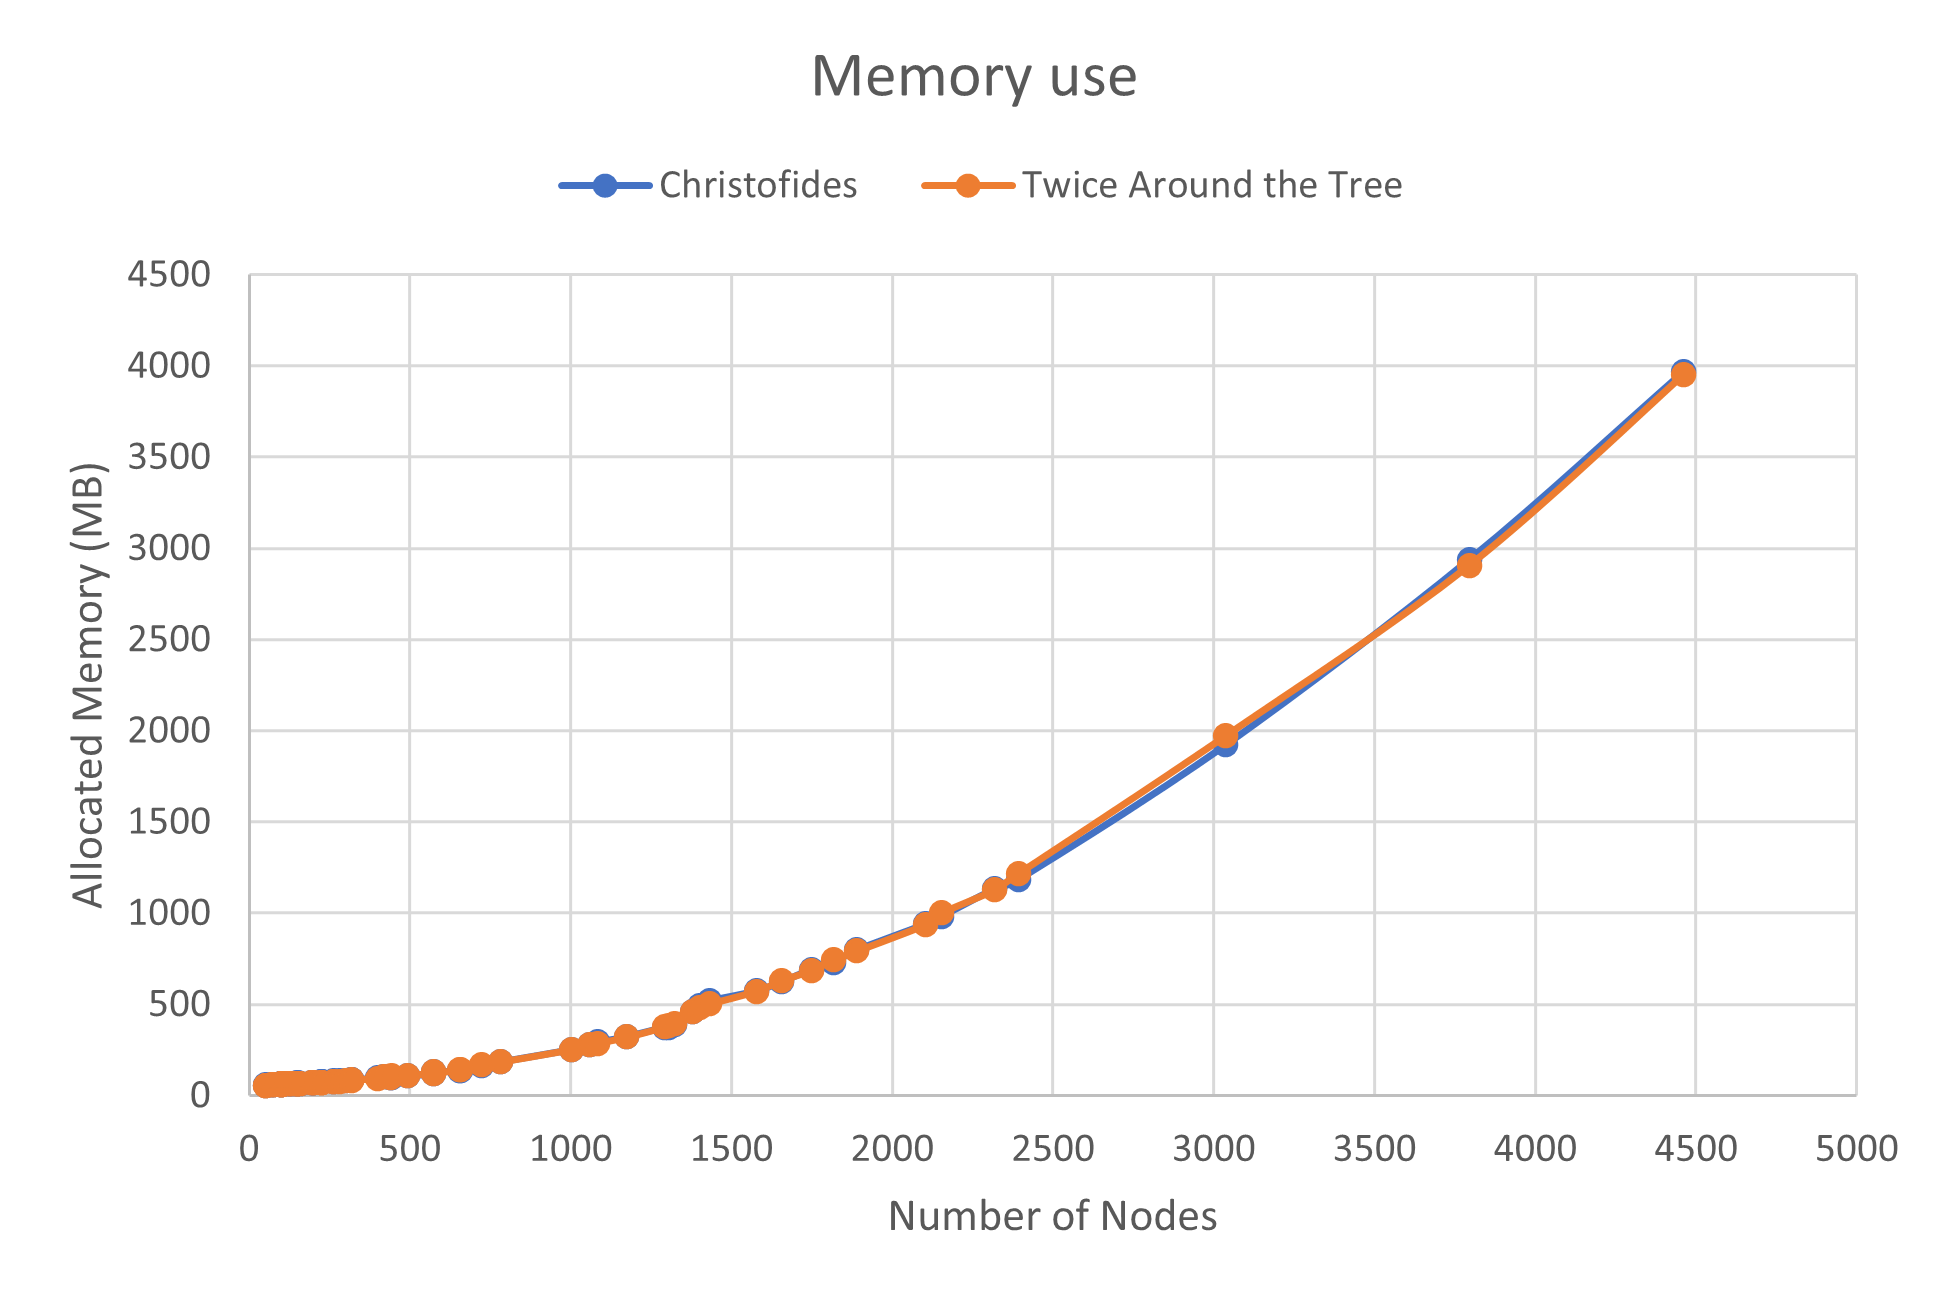
\includegraphics[height=.325\textheight]{memory_use_comparison.png}
\caption{Gráfico comparando a memória alocada entre os algoritmos de Christofides e Twice-around-the-tree.}
\label{fig:mem_use}
\end{figure}

O gráfico exibe uma pegada de memória semelhante para ambos os algoritmos. No entanto, para colocar as coisas em perspectiva, vamos analisar a Figura~\ref{fig:memory_behaviour}.

\begin{figure}[ht]
\centering
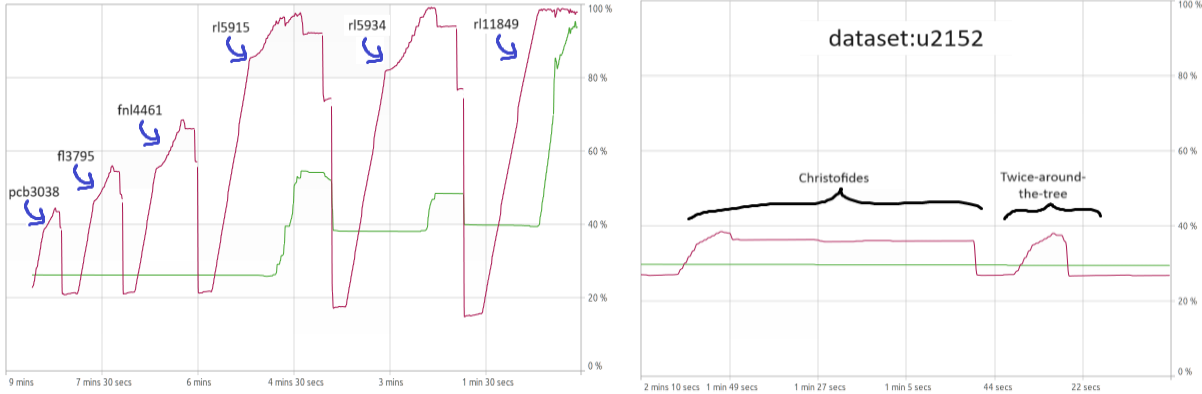
\includegraphics[width=\textwidth]{memory_profile_comparison.png}
\caption{(a) Gráfico mostrando o uso de memória para o algoritmo Twice-around-the-tree. (b) Gráfico mostrando o uso de memória para o algoritmo de Christofides.}
\label{fig:memory_behaviour}
\end{figure}

A primeira coisa que deve ser observada é que, para cada algoritmo, houve um conjunto de dados em que a memória alocada ultrapassou a capacidade de RAM disponível (consulte a Seção~\ref{sec:implementation} para as especificações do computador) e o armazenamento no arquivo \texttt{swap} \footnotemark foi acionado. Isso pode ser observado na execução do conjunto de dados \texttt{rl5915} com o Twice-around-the-tree, na Figura~\ref{fig:memory_behaviour} (a). Esse comportamento é semelhante no algoritmo de Christofides.

\footnotetext{\texttt{Swap} ou arquivo de página é uma seção de um disco rígido usada como local temporário para armazenar informações quando a RAM (memória de acesso aleatório) do computador está totalmente utilizada. Ele tem velocidades significativamente mais lentas em comparação com a memória principal.}

Em segundo lugar, a partir do conjunto de dados \texttt{rl11849}, o computador não tinha memória e \texttt{swap} suficientes para construir o grafo mesmo nas execuções sem monitoramento de memória (consulte a Figura~\ref{fig:memory_behaviour} (a)), causando o travamento do computador\footnotemark. Como o uso do \texttt{memory\_profiler} nos dá uma pegada de memória significativamente maior, a execução dos conjuntos de dados menores \texttt{rl5915} e \texttt{rl5934} com ele também não foi possível.

\footnotetext{Mesmo que o computador tenha travado ao atingir o uso máximo de RAM + \texttt{swap}, o estudante observou que, ao executar no Microsoft Windows em vez de Ubuntu em tais circunstâncias, não ocorreu travamento. Infelizmente, a máquina disponível com Windows era menos potente e levaria muito mais tempo.}

A Figura~\ref{fig:memory_behaviour} (b) exibe como a pegada de memória para ambos os algoritmos é bastante semelhante (usando um conjunto de dados pequeno para adequar a execução do algoritmo de Christofides).

O estudante não conseguiu implementar uma solução útil de branch-and-bound para comparar com as aproximações. Todas as tentativas, tanto em Python quanto em C++, causaram um uso explosivo de memória, travando o computador mesmo para o menor conjunto de dados. O estudante é obrigado a concluir que tentar resolver esse problema com essa abordagem não é prático no sentido absoluto, embora possa haver maneiras mais astutas e eficientes de implementação. No entanto, ele está seguro de que escolher o \textit{Depth-First-Search} foi a intuição correta.

\subsection{Qualidade da Solução} \label{sec:exp_quality}

O gráfico da Figura~\ref{fig:quality_ratio} mostra a razão $\frac{Solução Aproximada}{Solução Ótima}$.

\begin{figure}[ht]
\centering
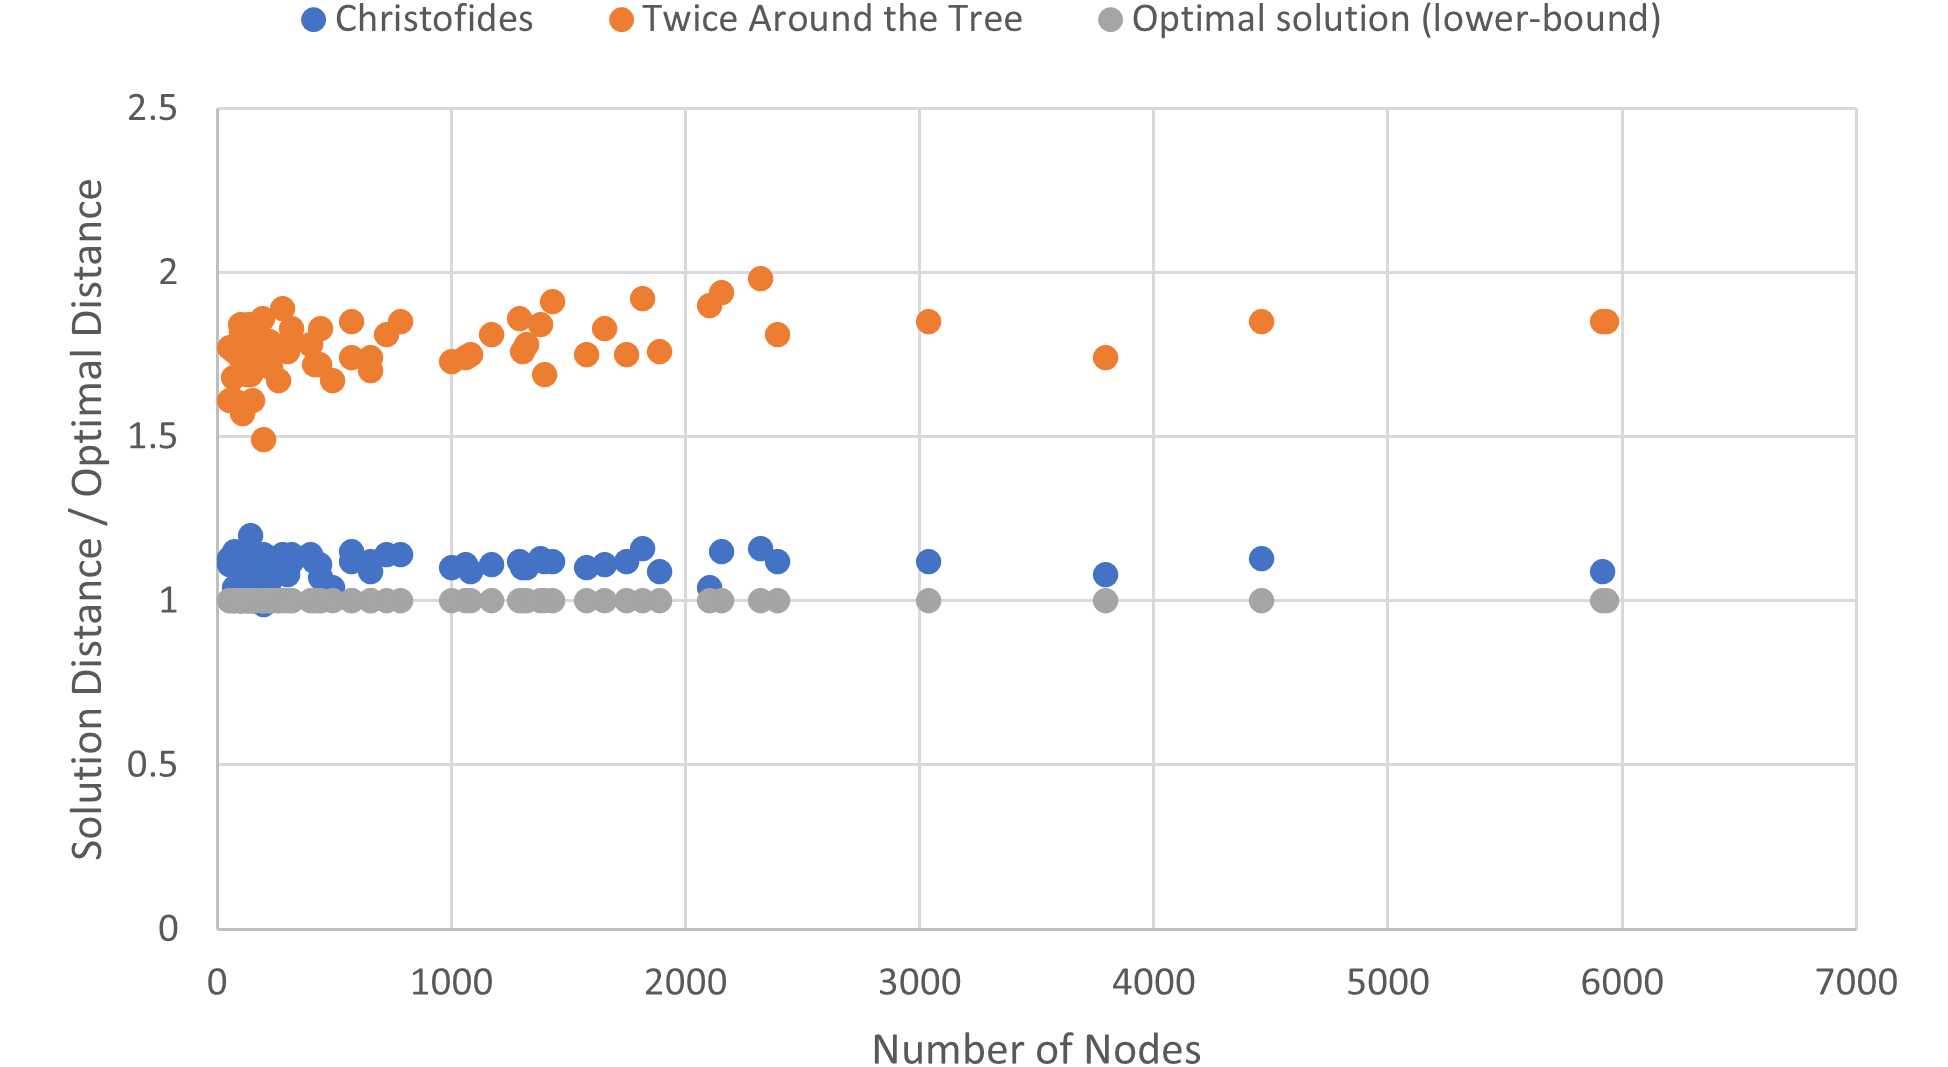
\includegraphics[height=.325\textheight]{quality_ratio.png}
\caption{Gráfico comparando a qualidade das soluções aproximadas e ótimas.}
\label{fig:quality_ratio}
\end{figure}

O Twice-around-the-tree permanece consistentemente abaixo do caso teórico pior esperado (Seção~\ref{sec:twice_explanation}) de duas vezes a solução ótima, e as soluções de Christofides encontram caminhos que são consistentemente melhores e mais próximos, mantendo também a estreita razão de qualidade de 1.5 especificada na Seção~\ref{sec:chris_explanation}.

\subsection{Tempo de Execução} \label{sec:exp_time}

O tempo de execução dos algoritmos pode ser comparado com a Figura~\ref{fig:exec_time}.

\begin{figure}[ht]
\centering
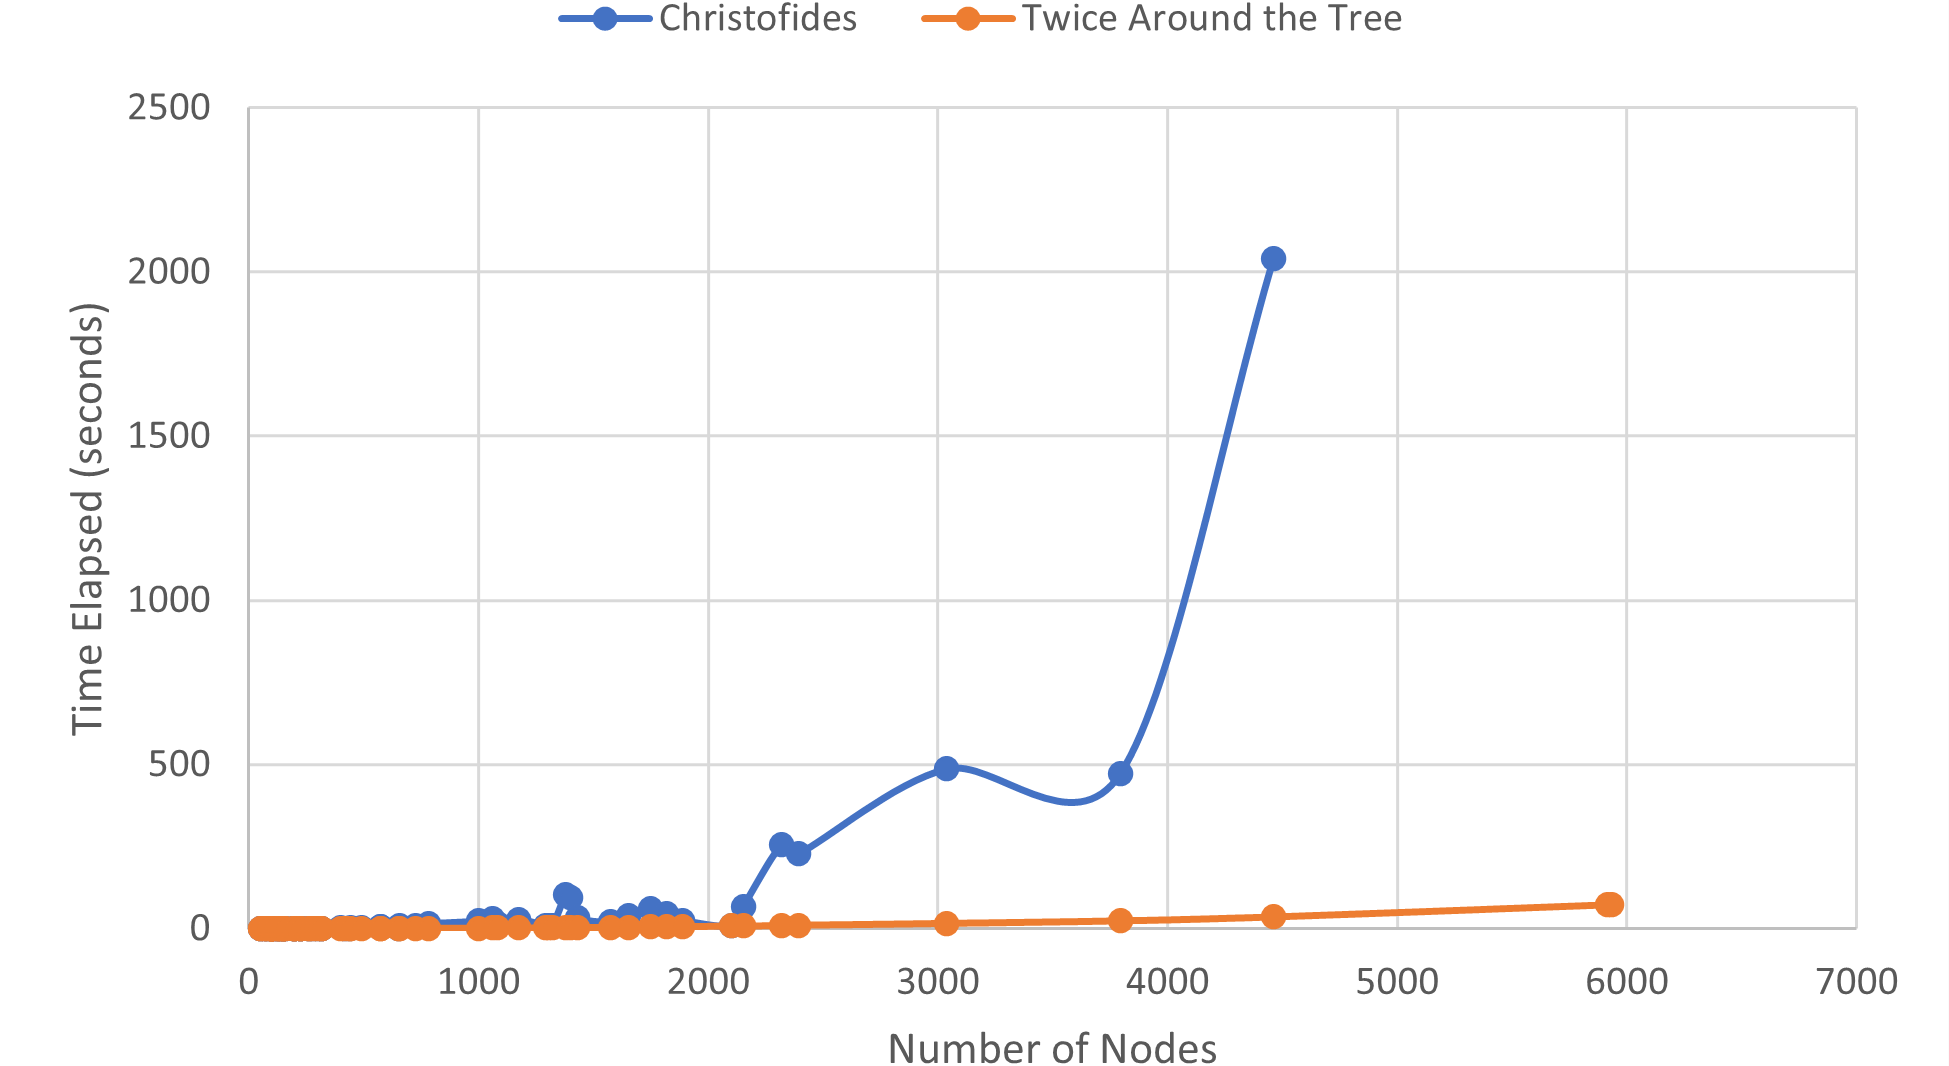
\includegraphics[height=.325\textheight]{execution_time_comparison.png}
\caption{Gráfico comparando o tempo decorrido entre os algoritmos de Christofides e Twice-around-the-tree.}
\label{fig:exec_time}
\end{figure}

O algoritmo de Christofides leva significativamente mais tempo para ser executado em comparação com o Twice-around-the-tree. Na verdade, parece formar um crescimento exponencial, mas isso deve ser colocado em perspectiva, já que o estudante diagnosticou que os algoritmos ultrapassaram a memória RAM disponível (consulte a Seção~\ref{sec:exp_memory}). Este fato pode explicar por que o \texttt{fnl4461} mostrou um aumento tão drástico no tempo de execução: o uso de memória \texttt{swap} o retardou, e a partir deste ponto em diante, o gráfico não exibirá seu comportamento ideal. Em outras palavras, isso não constitui evidência de que o algoritmo de Christofides seja exponencial (consulte a Seção~\ref{sec:chris_explanation}).

Isso ilustra perfeitamente como é difícil otimizar algoritmos exponenciais, mesmo para casos relativamente pequenos. O Twice-around-the-tree, apesar de ter uma qualidade muito pior do que o Christofides, é significativamente mais rápido e deve fornecer respostas suficientemente boas para as situações certas.

\section{Conclusões} \label{sec:conclusions}

Implementar os algoritmos proporcionou insights valiosos sobre os aspectos do mundo real de resolver o TSP. Isso demonstrou as compensações entre qualidade da solução, tempo de execução e requisitos de memória, e destacou as limitações de algoritmos exponenciais, já que a técnica de branch-and-bound pode rapidamente se tornar intratável mesmo para instâncias relativamente pequenas do problema.

Para as aproximações, o algoritmo de Christofides consistentemente supera o algoritmo Twice-around-the-tree em termos de qualidade da solução, mantendo uma estreita razão de qualidade de 1.5 com a solução ótima. No entanto, é significativamente mais lento. O algoritmo Twice-around-the-tree, por outro lado, oferece uma compensação razoável entre qualidade da solução e tempo de execução.

Os resultados sugerem que o algoritmo Twice-around-the-tree é uma boa escolha para aplicações práticas do TSP, pois fornece um equilíbrio razoável entre qualidade e eficiência. O algoritmo de Christofides pode ser usado quando é necessária uma solução de alta qualidade, mas é importante estar ciente de suas limitações computacionais.

\bibliographystyle{sbc}
\bibliography{sbc-template}

\end{document}